\documentclass{article}
\usepackage{fancyhdr}
\usepackage{titlesec}
\usepackage{graphicx}
\graphicspath{ {./img/} }
\usepackage{multirow}

\pagestyle{fancy}
\fancyhf{}
\lhead{Modul 6 Praktikum Jaringan Komputer}
\rfoot{\footnotesize Page \thepage}
\lfoot{\footnotesize Mahyus Ihsan, S.Si, M.Si \newline Jurusan Informatika Universitas Syiah Kuala \newline Modul oleh : Diky Wahyudi, Furqan Al Ghifari, Rendika Rahmaturrizki}
\renewcommand{\headrulewidth}{1pt}
\renewcommand{\footrulewidth}{1pt}

\titleformat*{\section}{\small\bfseries}

\begin{document}
    \begin{center}
        \textbf{Modul 6 Praktikum Jaringan Komputer}

        \textbf{ICMP dan Basic Router Configuration}
    \end{center}

    \section*{Deskripsi Singkat}
    \begin{flushleft}
        Internet Control Message Protocol (ICMP) adalah  jaringan protokol yang bertanggung jawab untuk melaporkan kesalahan melalui cara menghasilkan dan mengirim pesan ke alamat IP sumber ketika ada masalah jaringan pada sistem. 
    \end{flushleft}

    \section*{Tujuan}
    \begin{enumerate}
        \item Dapat memahami tentang ICMP dan cara kerjanya
        \item Dapat melakukan konfigurasi dasar pada sebuah router
    \end{enumerate}

    \begin{flushleft}
        \textbf{Materi 1 - ICMP}
        \newline

        Internet Control Message Protocol atau biasa disingkat ICMP adalah protokol jaringan yang berguna untuk memecahkan berbagai masalah terkait konektivitas. Protokol ini digunakan oleh berbagai perangkat jaringan, seperti router, modem, server, dan yang lainnya.
        \newline

        Sederhananya, ICMP digunakan untuk pelaporan error dengan menentukan apakah data mencapai tujuan yang dimaksudkan dengan relatif cepat atau tidak.

        Berikut adalah fungsi utama ICMP : 

        \begin{itemize}
            \item Izinkan router untuk memberi tahu sumber ketika paket IP yang dikirim oleh sumber tidak dapat dikirim.
            \item Izinkan sumber menemukan semua jalur yang tersedia ke perangkat tujuan.
            \item Izinkan sumber untuk memeriksa apakah perangkat tujuan online dan up.
            \item Izinkan administrator untuk menguji konektivitas dan men-debug masalah terkait konektivitas.
        \end{itemize}

        Berikut adalah pesan error dari protokol ICMP : 

        \begin{enumerate}
            \item \textbf{Destination Unreachable}
            \newline
            Penyebab utamanya adalah jalur fisik dan logic yang terputus sehingga tidak bisa mencapai host tujuan.

            \item \textbf{Time Exceeded}
            \newline
            Secara sederhana, pesan ini akan muncul apabila kehabisan waktu. Kondisi yang memicunya yaitu saat field Time To Live (TTL) sudah mencapai waktu yang ditargetkan padahal paket belum berhasil diteruskan. 
            Sama halnya ketika Anda mengakses laman website namun akhirnya gagal dimuat dan muncul notifikasi 'Request Timed Out'.

            \item \textbf{Parameter Problem}
            \newline
            Pesan ini berkaitan dengan kesalahan pada header tiap paket yang akan dikirimkan.

            \item \textbf{Source Quench}
            \newline
            Protokol ICMP akan mengirimkan source quench apabila network tujuan sedang kelebihan beban sehingga mempengaruhi performanya.

            \item \textbf{Redirect}
            \newline
            Kategori pesan ini muncul apabila transmisi data melalui rute yang salah. Sehingga akan dialihkan ke rute yang seharusnya.
        \end{enumerate}

        Kategori dalam ICMP Query Message terdiri dari:

        \begin{enumerate}
            \item 'Timestamp dan Timestamp Reply' berisi informasi mengenai estimasi waktu agar host tujuan dapat memproses paket data
            \item  'Echo dan Echo Reply' akan muncul untuk memastikan sistem tujuan masih aktif dengan menggunakan program ping. Nantinya, responden harus menjawab dengan data yang sama persis
            \item 'Address Mask' memuat jumlah netmask yang dibutuhkan oleh host dalam jaringan komputer.
        \end{enumerate}
    \end{flushleft}

    \begin{flushleft}
        \textbf{Materi 2 - Basic Router Configuration - Initial Router Settings}
        \newline

        \begin{enumerate}
            \item Bukalah modul \textbf{3.1 Packet Tracer - Configure Initial Router Settings.pka}
            
            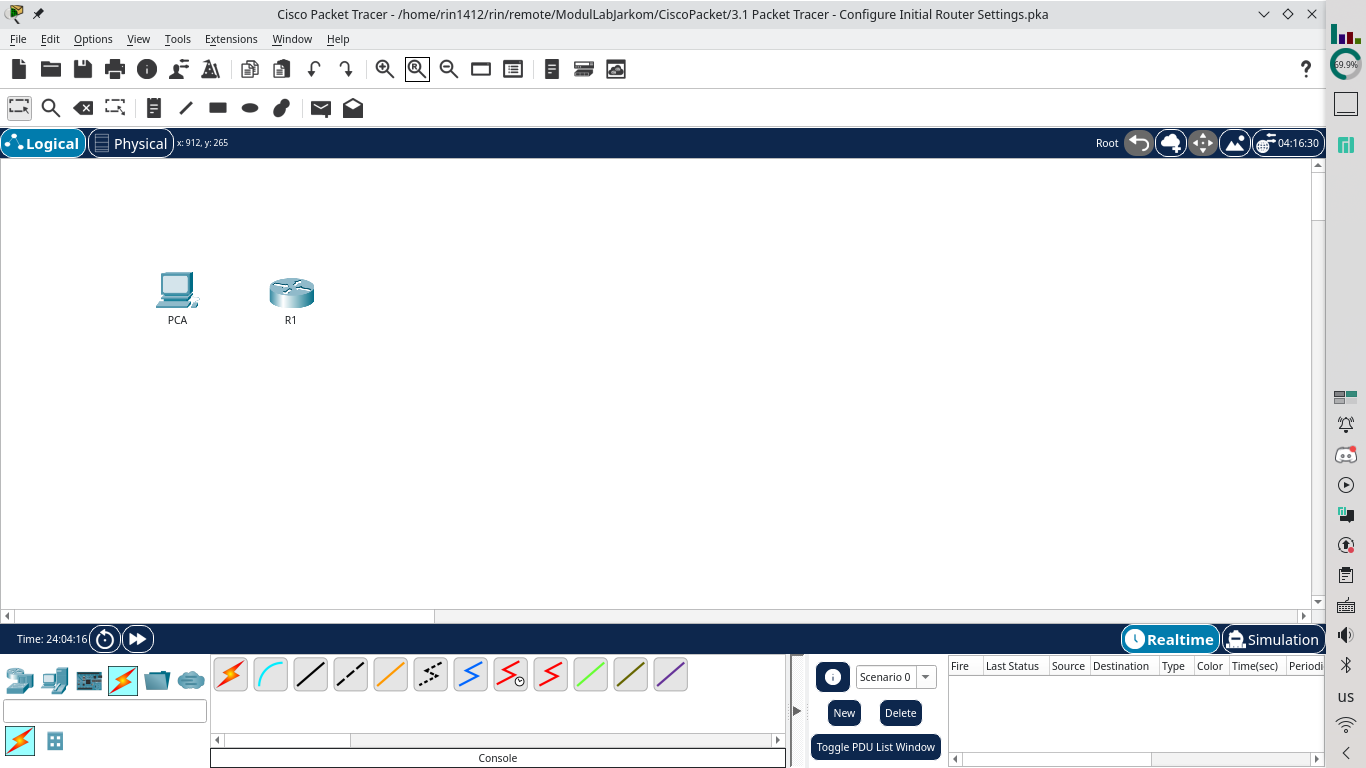
\includegraphics[scale=0.25]{2-1.png}

            \item Sambungkan PCA dengan Router menggunakan kabel console
            
            \begin{center}
                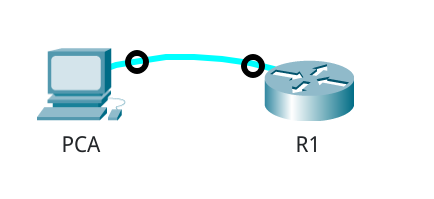
\includegraphics[scale=0.3]{2-2.png}
            \end{center}

            \item Buka terminal pada PCA, terminal berada pada menu \textbf{Desktop $>$ Terminal}

            \begin{center}
                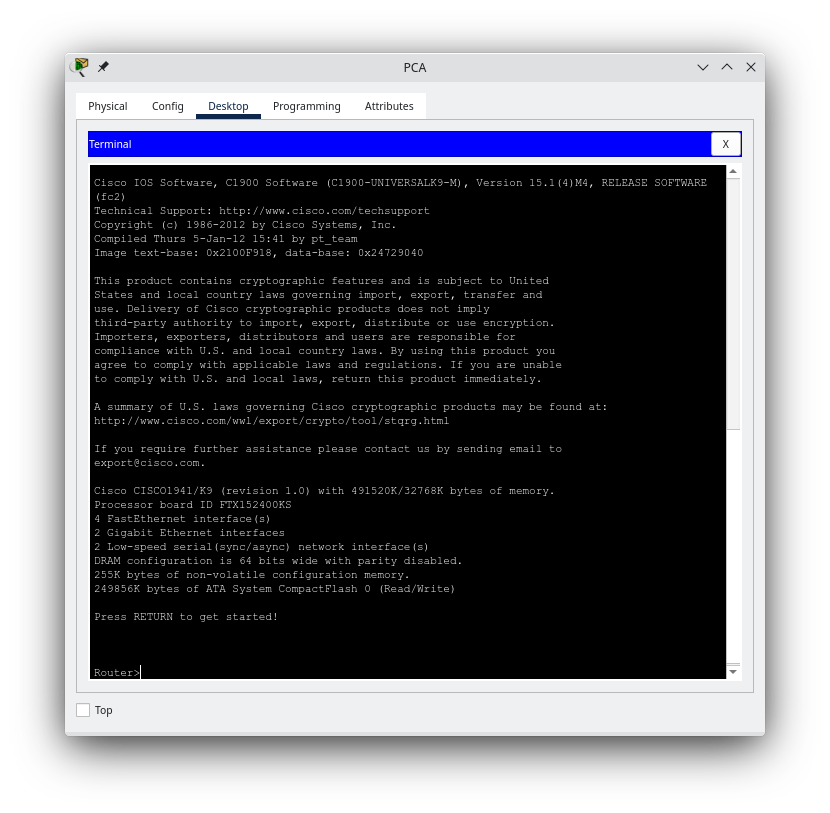
\includegraphics[scale=0.4]{2-3.png}
            \end{center}

            \item Masukklah ke dalam mode konfigurasi

            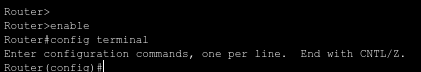
\includegraphics[]{2-4.png}

            \item Kemudian berikan hostname pada router

            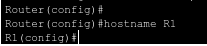
\includegraphics[]{2-5.png}

            \item Berikan password pada \textbf{line console 0} agar tidak semua orang dapat melakukan konfigurasi router.
            
            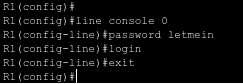
\includegraphics[]{2-6.png}

            \item Enable password dan secret agar tidak semua orang dapat masuk kedalam \textbf{User Exec Mode} ataupun \textbf{Privileged EXEC Mode}
            
            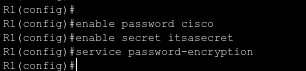
\includegraphics[]{2-7.png}

            \item Kemudian tambahkan banner motd

            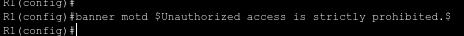
\includegraphics[scale=0.9]{2-8.png}

            \item Dan langkah terakhir lakukan copy dari running-config ke startup-config agar ketika router dimatikan konfigurasi yang tersimpan di dalam dapat dijalankan kembali pada saat router dihidupkan kembali.
            
            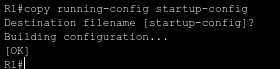
\includegraphics[]{2-9.png}

            \item Maka konfigurasi awal router sudah selesai.
        \end{enumerate}
    \end{flushleft}

    \begin{flushleft}
        \textbf{Materi 3 - Basic Router Configuration - Routing}
        \newline

        \begin{enumerate}
            \item Buatlah jaringan seperti pada gambar berikut : 
            
            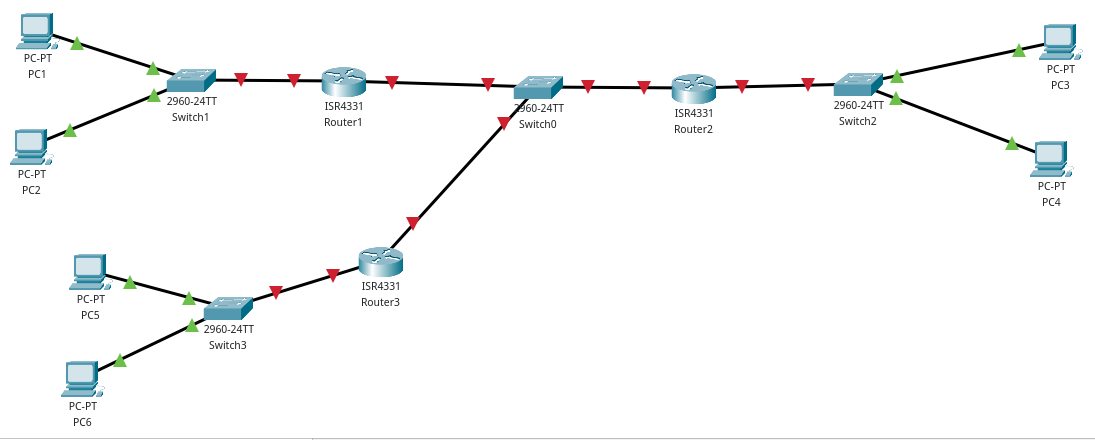
\includegraphics[scale=0.3]{1-1.png}

            \begin{tabular}{|c|c|c|c|}
                \hline
                Device & IP & Destination & Network \\
                \hline
                \multirow{2}{4em}{Router1} & 192.168.1.1/29 & Switch0 & 192.168.1.0/29\\
                & 192.168.1.9/29 & Switch1 & 192.168.1.8/29 \\
                \hline
                \multirow{2}{4em}{Router2} & 192.168.1.2/29 & Switch0 & 192.168.1.0/29\\
                & 192.168.1.17/29 & Switch2 & 192.168.1.16/29 \\
                \hline
                \multirow{2}{4em}{Router3} & 192.168.1.3/29 & Switch0 & 192.168.1.0/29\\
                & 192.168.1.25/29 & Switch3 & 192.168.1.24/29 \\
                \hline
                PC1 & 192.168.1.10 & - & 192.168.1.8 \\
                \hline
                PC2 & 192.168.1.11 & - & 192.168.1.8 \\
                \hline
                PC3 & 192.168.1.18 & - & 192.168.1.16 \\
                \hline
                PC4 & 192.168.1.19 & - & 192.168.1.16 \\
                \hline
                PC5 & 192.168.1.26 & - & 192.168.1.24 \\
                \hline
                PC6 & 192.168.1.27 & - & 192.168.1.24 \\
                \hline
            \end{tabular}

            \item Berikan IP pada masing-masing PC sesuai dengan tabel yang telah diberikan, dan jangan lupa untuk memasukkan default gateway pada setiap host pada network yang ada. Serta jangan lupa untuk mengecek konektivitas antar host pada setiap jaringan dengan menggunakan perintah \textbf{ping}

            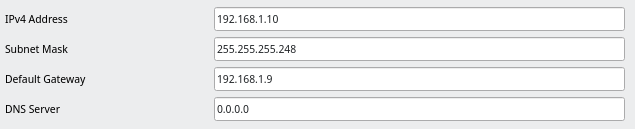
\includegraphics[scale=0.6]{1-2.png}
            Contoh Konfigurasi IP PC1

            \item Berikan IP pada masing - masing Switch dengan melakukan konfigurasi pada masing - masing router.

            Router1 ke Switch1
            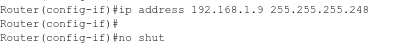
\includegraphics[]{1-4.png}

            Router2 ke Switch2
            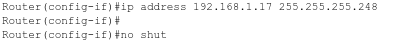
\includegraphics[]{1-5.png}

            Router3 ke Switch3
            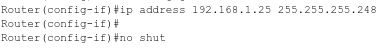
\includegraphics[]{1-6.png}

            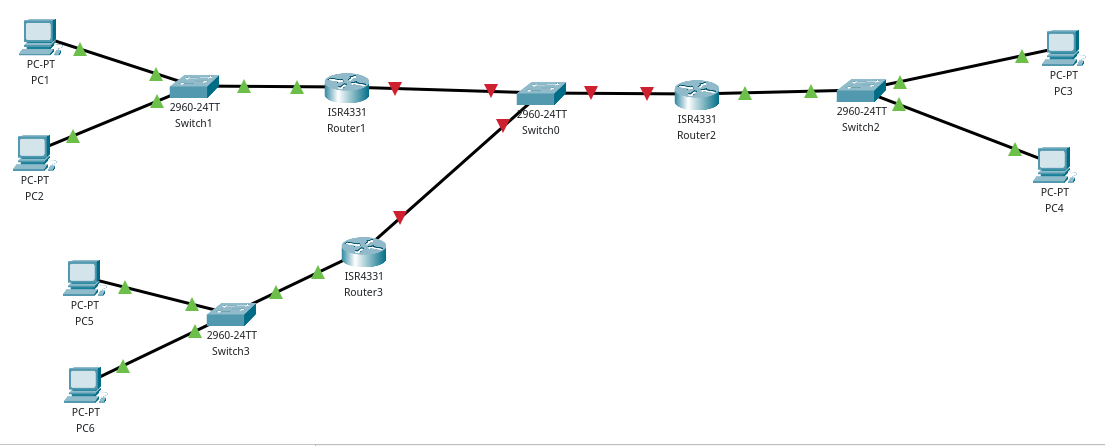
\includegraphics[scale=0.3]{1-7.png}
            Setelah memberikan IP pada jalur menuju Switch maka setiap router dan Switch menuju ke setiap Network telah tersambung dan berwarna hijau 

            \item Setelah menyambungkan Router dengan Switch pada setiap network, langkah selanjutnya adalah mengkoneksikan setiap router ke Switch0 dan melakukan \textit{static routing}
            
            Router1 ke Switch0
            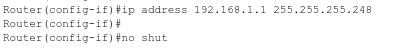
\includegraphics[]{1-8.png}

            Router2 ke Switch0
            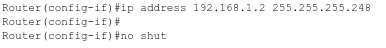
\includegraphics[]{1-9.png}

            Router3 ke Switch0
            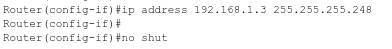
\includegraphics[]{1-10.png}

            Setelah terhubung maka akan menjadi seperti ini

            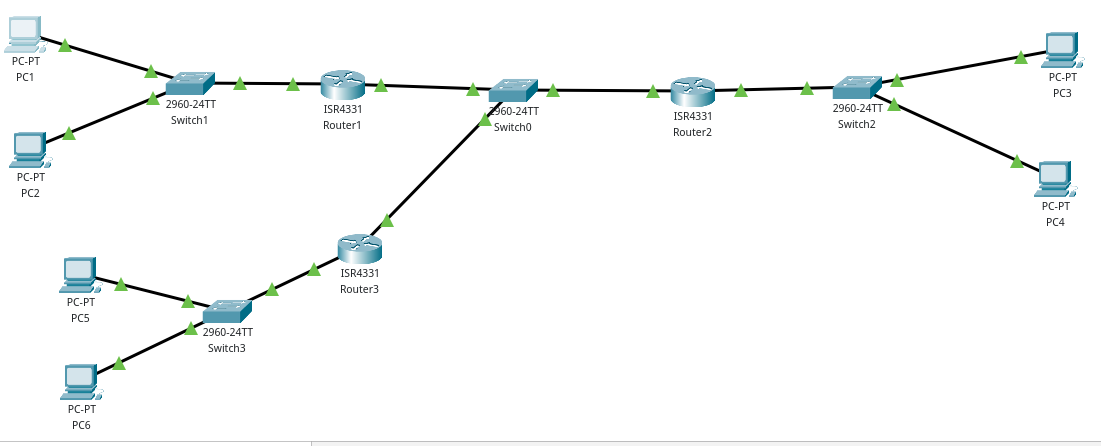
\includegraphics[scale=0.3]{1-11.png}

            \item Setelah menghubungkan setiap Router ke Switch0, cobalah melakukan ping dari suatu host ke host lain yang berada pada network yang beda. Contoh ping dari PC1 ke PC4
            
            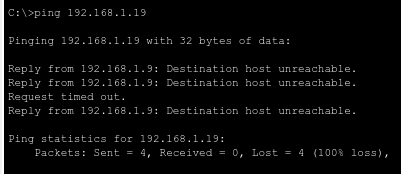
\includegraphics[scale=0.7]{1-12.png}

            Dan terlihat bahawa pesan ICMP mengembalikan pesan Destination host Unreachable. Hal ini terjadi karena router belum dilakukan konfigurasi \textit{static routing}

            \item Hubungkan setiap network dengan melakukan \textit{static routing} pada setiap router. Untuk melakukan static routing pada router bisa menggunakan perintah 
            
            \begin{center}
                \textbf{\#ip route [destination] [subnet] [next hop address]}
            \end{center}

            Routing pada Router1
            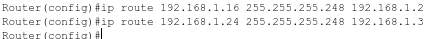
\includegraphics[scale=0.9]{1-13.png}

            Routing pada Router2
            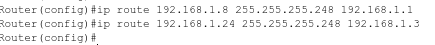
\includegraphics[scale=0.9]{1-14.png}

            Routing pada Router3
            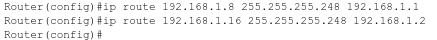
\includegraphics[scale=0.9]{1-15.png}

            \item Setelah melakukan routing maka lakukan kembali ping dari suatu host ke host lain yang berada pada network yang beda. Contoh ping dari PC1 ke PC4
            
            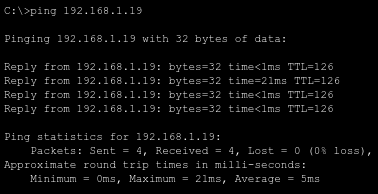
\includegraphics[scale=0.7]{1-16.png}

            Dan PC1 mendapatkan reply dari PC4, sehingga sekarang setiap network sudah saling terhubung.
        \end{enumerate}
    \end{flushleft}
\end{document}
